\documentclass{beamer}

\mode<presentation>
{
  \usetheme{Warsaw}
  \setbeamercovered{transparent}
}

\usepackage[english]{babel}
\usepackage[utf8]{inputenc}
\usepackage{times}
\usepackage[T1]{fontenc}
\usepackage{graphicx}
\graphicspath{ {images/} }

\title[]
{Dependency injection}

\author[Adrian Mularczyk]{Adrian Mularczyk}

\institute[PGS Softwarei]
{
PGS Software
}

\date{}

\begin{document}

\begin{frame}
  \titlepage 
\end{frame}

\begin{frame}{Agenda}
  \tableofcontents
\end{frame}

\section{Description of the problem}

\begin{frame}{}
\begin{center}
\Huge{Description of the problem}
\end{center}
\end{frame}

\subsection*{SOLID}

\begin{frame}{SOLID}
\begin{table}
     \begin{Large}
	\begin{tabular}{ c c c l }
	S &-& SRP& (Single responsibility principle)\\
	O &-& OCP& (Open/closed principle)\\
	L &-& LSP& (Liskov substitution principle)\\
	I &-& ISP& (Interface segregation principle)\\
	D &-& DIP& (Dependency inversion principle)
	\end{tabular}
     \end{Large}
\end{table}
\end{frame}

\begin{frame}{SOLID}
\begin{table}
     \begin{Large}
	\begin{tabular}{ c c c l }
\color{gray} S &\color{gray}-& \color{gray}SRP& \color{gray}(Single responsibility principle)\\
\color{gray} O &\color{gray}-& \color{gray}OCP& \color{gray}(Open/closed principle)\\
\color{gray}	L &\color{gray}-& \color{gray}LSP& \color{gray}(Liskov substitution principle)\\
\color{gray}	I &\color{gray}-& \color{gray}ISP& \color{gray}(Interface segregation principle)\\
	D &-& DIP& (Dependency inversion principle)
	\end{tabular}
     \end{Large}
\end{table}
\end{frame}

\begin{frame}{Dependency Inversion Principal}
\begin{figure}
	\begin{center}
  		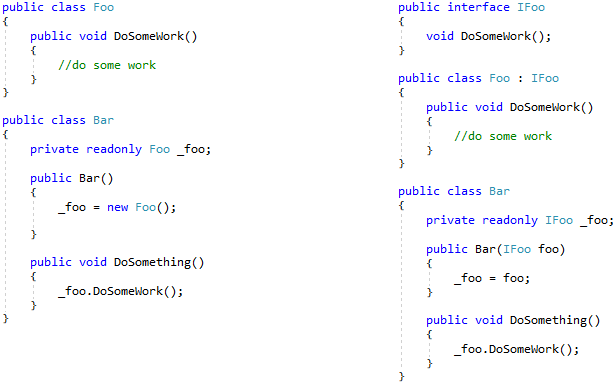
\includegraphics[height=6cm]{PresentationDIP.png}
	\end{center}
\end{figure}
\end{frame}

\subsection*{Dependency injection container}
\begin{frame}{Dependency injection container}
\begin{center}
\Large{Dependency injection container}
\end{center}
\end{frame}

\begin{frame}{Dependency injection container}
\begin{table}
     \begin{Large}
	\begin{tabular}{ p{6cm} p{6cm} }
		\begin{minipage}{.6\textwidth}
			\begin{itemize}
				\item Register
				\item Resolve
			\end{itemize}
   		 \end{minipage}
   		 &
	\end{tabular}
     \end{Large}
\end{table}
\end{frame}

\begin{frame}{Dependency injection container}
\begin{table}
	\begin{tabular}{ p{5cm} p{5cm} }
		\begin{minipage}{.5\textwidth}
  			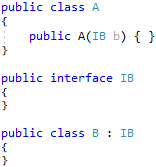
\includegraphics[height=2.8cm]{Example_Container.png}
   		 \end{minipage}
   		 &
		\begin{minipage}{.5\textwidth}
			{\tiny \texttt{container.Register<A>();\\
				container.Register<IB, B>();}}\\ \\
			{\tiny \texttt{container.Resolve<IB>();\\
				container.Resolve<A>();}}
   		 \end{minipage}
	\end{tabular}
\end{table}
\end{frame}


\section{Dependency injection}

\begin{frame}{}
\begin{center}
\Huge{Dependency injection}
\end{center}
\end{frame}

\subsection*{Dependency injection}

\begin{frame}{Dependency injection}
     \begin{Large}
	\begin{itemize}
		\item Injecting by the constructor
		\item Injecting by the method
		\item Injecting by the property
	\end{itemize}
     \end{Large}
\end{frame}

\begin{frame}{Dependency injection}
\begin{table}
	\begin{tabular}{ p{5cm} p{5cm} }
		\begin{minipage}{.5\textwidth}
  			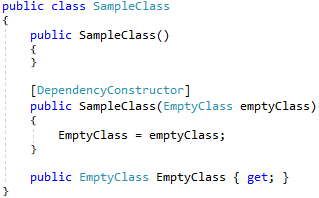
\includegraphics[height=3cm]{DependencyConstructor.png}
   		 \end{minipage}
   		 &
		\begin{minipage}{.5\textwidth}
  			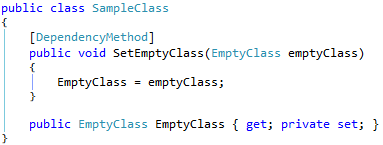
\includegraphics[height=2cm]{DependencyMethod.png} \\ \\
  			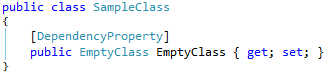
\includegraphics[height=1cm]{DependencyProperty.png}
   		 \end{minipage}
	\end{tabular}
\end{table}
\end{frame}

\subsection*{Registration types}

\begin{frame}{Registration types}
     \begin{Large}
	\begin{itemize}
		\item Register as Singleton,
		\item Register as Transient,
		\item Register as Scope (Thread, HttpRequest),
		\item Register as FactoryMethod.
	\end{itemize}
     \end{Large}
\end{frame}

\subsection*{Sample implementations}

\begin{frame}{Sample implementations}
\begin{table}
	\begin{tabular}{ p{5cm} p{5cm} }
	
	\begin{minipage}{.5\textwidth}
\Large{\begin{itemize}
	\item NInject
	\item Unity
	\item Autofac
	\item StructureMap
	\item Windsor
\end{itemize}}
   	 \end{minipage}
   	 &
	\begin{minipage}{.5\textwidth}
\Large{\begin{itemize}
	\item Grace
	\item DryIoc
	\item LightInject
	\item SimpleInjector
\end{itemize}}
   	 \end{minipage}

	\end{tabular}
\end{table}
http://www.palmmedia.de/blog/2011/8/30/ioc-container-benchmark-performance-comparison
\end{frame}


\section{Code}

\begin{frame}{}
\begin{center}
\Huge{Code}
\end{center}
\end{frame}

\subsection*{Usage}
\begin{frame}{Adding DI to our project}
\begin{center}
\Large{\begin{itemize}
	\item .NET Framework
	\item .NET Core
\end{itemize}}
\end{center}
\end{frame}

\subsection*{Sample implementation}
\begin{frame}{Sample implementation}
\begin{center}
\Huge{Demo}
\end{center}
\end{frame}

\subsection*{Extensions}
\begin{frame}{Extensions}
\begin{center}
\Large{\begin{itemize}
	\item List instead Dictionary
	\item Many destination types
	\item Many input types
\end{itemize}}
\end{center}
\end{frame}	


\section{Summary}

\begin{frame}{}
\begin{center}
\Huge{Summary}
\end{center}
\end{frame}

\begin{frame}{Questions?}
\begin{center}
\Huge{Thank you!}\\
\Large{e-mail: amularczyk@pgs-soft.com}
\end{center}
\end{frame}


\end{document}